\section{Chapter 9 -- Threads}
\subsection{Defining, Instantiating and Starting Threads}
In java, a `thread' means two different things:
\begin{itemize}
    \item An instance of the class \verb#java.lang.Thread#
    \item A thread of execution
\end{itemize}
An instance of \verb#Thread# is just an object. Like any other object in java, 
it has variables and methods and lives and dies on the heap. A thread of 
execution is an individual process (a `lightweight' process) that has its own 
call stack. In java, there is one thread per call stack -- or (equivalently) 
one call stack per thread.

The JVM, which gets its turn at the CPU by whatever scheduling mechanism the 
underlying OS uses, operates like a mini-OS and schedules its own threads 
regardless of the underlying OS. The most important concept to understand from 
this chapter is that when it comes to threads, very little is guaranteed

\subsection{Making a Thread}
A thread in java begins as an instance of \verb#java.lang.Thread#. You'll find 
methods in the Thread class for managing threads including creating, starting, 
and pausing them. For the exam, you'll need to know, at a minimum, the 
following methods:
\begin{itemize}
    \item \verb#start()#
    \item \verb#yield()#
    \item \verb#sleep()#
    \item \verb#run()#
\end{itemize}
You can define and instantiate a thread in one of two ways:
\begin{itemize}
    \item Extend the \verb#java.lang.Thread# class
    \item Implement the \verb#java.lang.Runnable# interface
\end{itemize}

\subsection{Defining a Thread}
\subsubsection{Extending java.lang.Thread}
The simplest way to define code to run in a separate thread is to:
\begin{enumerate}
    \item Extend the \verb#java.lang.Thread# class
    \item Override the \verb#run()# method
\end{enumerate}
\begin{verbatim}
    class MyThread extends Thread {
        public void run() {
            System.out.println("job running in MyThread");
        }
    }
\end{verbatim}
Note that you can overload (in addition to overriding) the \verb#run()# method in the \verb#Thread# subclass

\subsubsection{Implementing java.lang.Runnable}
Implementing the \verb#Runnable# interface gives you a way to extend from any class, but still define behaviour that will be run by a separate thread.
\begin{verbatim}
    class MyRunnable implements Runnable {
        public void run() {
            System.out.println("job running in MyRunnable");
        }
    }
\end{verbatim}

\subsection{Instantiating a Thread}
If you extend the \verb#Thread# class, instantiation is simple:
\begin{verbatim}
    MyThread thread = new MyThread();
\end{verbatim}
If you implement \verb#Runnable#, instantiation is only slightly less simple. First, you instantiate your \verb#Runnable# class, and then instantiate a thread, giving it the instance of \verb#Runnable#:
\begin{verbatim}
    MyRunnable runnable = new MyRunnable();
    Thread thread = new Thread(runnable);
\end{verbatim}
If you create a thread using the no-arg constructor, the thread will call its own \verb#run()# method when it is time to start working. That is exactly what you want when you extend \verb#Thread#, but when you use \verb#Runnable#, you need to tell the new thread to use your \verb#run()# method rather than its own. The \verb#Runnable# you pass to the \verb#Thread# constructor is called the target or the target Runnable.

You can pass a single \verb#Runnable# instance to multiple \verb#Thread# objects, so that the same \verb#Runnable# becomes the target of multiple threads.

Note that the \verb#Thread# class itself implements \verb#Runnable#. This means you can pass a \verb#Thread# to another \verb#Thread#'s constructor:
\begin{verbatim}
    Thread thread = new Thread(new MyThread());
\end{verbatim}

Besides the no-arg constructor and the constructor that takes a \verb#Runnable# denoting the target Runnable, there are other overloaded \verb#Thread# constructors:
\begin{itemize}
    \item \verb#Thread()#
    \item \verb#Thread(Runnable target)#
    \item \verb#Thread(Runnable target, String name)#
    \item \verb#Thread(String name)#
\end{itemize}
When a thread has been instantiated but not started (in other words, the \verb#start()# method has not been invoked on the \verb#Thread# instance), the thread is said to be in the `new' state. At this stage, the thread is not yet considered to be `alive'. Once the \verb#start()# method is called, the thread is considered to be `alive' (even though the \verb#run()# method may not have actually started executing yet). A thread is considered `dead' (no longer `alive') after the \verb#run()# method completes. The \verb#isAlive()# method is the best way to determine if a thread has been started but has not completed its \verb#run()# method. Note that the \verb#getState()# method is very useful for debugging, but it not needed for the exam

\subsection{Starting a Thread}
To start a thread, invoke the \verb#start()# method. When \verb#start()# is called:
\begin{itemize}
    \item A new thread of execution starts (with a new call stack)
    \item The tread moves from the `new' state to the `runnable' state
    \item When the thread gets a chance to execute, its target \verb#run()# method will run
\end{itemize}

There is nothing special about the \verb#run()# method. Calling a \verb#run()# 
method directly just means you are invoking a method from whatever thread is 
currently executing, and the \verb#run()# method goes onto the current call 
stack rather than at the beginning of a new call stack. The following does not 
start a new thread of execution:
\begin{verbatim}
    Thread thread = new Thread();
    t.run();    // legal, but does not start a new thread
\end{verbatim}

Note that the \verb#Thread.currentThread().getName()# method can be used to obtain the name of the currently executing thread

\subsubsection{Starting and Running Multiple Threads}
Note that there is nothing in the java specification that says threads will start running in the order in which they were started (in other words, the order in which \verb#start()# was invoked on each thread). There is no guarantee that once a thread starts executing, it will keep executing until it is done. Within each thread, things will happen in a predictable order. However, the actions of different threads can mix together in unpredictable ways.

Just because a series of threads are started in a particular order, doesn't mean they will run in this order. For any group of started threads, order and duration is not guaranteed by the scheduler. You do not know for example, if one thread will run to completion before the others have a chance to get in, or whether they will all take turns nicely, or whether they will do a combination of both. There is a way, however, to start a thread but tell it not to run until some other thread has finished. You can do this with the \verb#join()# method.

Notes on threads:
\begin{itemize}
    \item A \verb#Thread# is done being a thread of execution when its target \verb#run()# method completes
    \item Once a \verb#Thread# has been started, it can never be started again. If you have a reference to a \verb#Thread#, and you call \verb#start()#, it is started. If you call \verb#start()# again, it will cause an \verb#IllegalThreadStateException#, which is a kind of \verb#RuntimeException#. This happens regardless of whether the \verb#run()# method has completed from the first \verb#start()# call. Only a new \verb#Thread# can be started, and then only once
\end{itemize}

\subsubsection{The Thread Scheduler}
The thread scheduler is the part of the JVM (although most JVMs map java 
threads directly to native threads on the underlying OS) that decides which 
thread should run at any given time, and also takes threads out of the 
`running' state.

Any thread in the `runnable' state can be chosen by the scheduler to be the one 
and only running thread. The order in which `runnable' threads are chosen to 
run is not guaranteed. Although we don't control the thread scheduler (we 
cannot for example, tell a specific thread to run), we can sometimes influence 
it

\subsubsection{Methods from the java.lang.Thread Class}
Some of the methods that can help in influencing thread scheduling are:
\begin{itemize}
    \item \verb#public static void sleep(long millis) throws InterruptedException#
    \item \verb#public static void yield()#
    \item \verb#public final void join() throws InterruptedException#
    \item \verb#public final void setPriority(int newPriority)#
\end{itemize}
Note that both \verb#sleep()# and \verb#join()# have overloaded versions not 
listed above

\subsubsection{Methods from the java.lang.Object Class}
Every class in java inherits the following three thread-related methods:
\begin{itemize}
    \item \verb#public final void wait() throws InterruptedException#
    \item \verb#public final void notify()#
    \item \verb#public final void notifyAll()#
\end{itemize}
The \verb#wait()# method has three overloaded versions (including the one 
listed above)

\subsection{Thread States and Transitions}
\subsubsection{Thread States}
A thread can be only in one of five states:
\begin{itemize}
    \item New -- This is the state a thread is in after the \verb#Thread# 
    instance has been created, but the \verb#start()# method has not been 
    invoked on the thread. It is a live \verb#Thread# object, but not yet a 
    thread of execution. At this point, the thread is considered `not alive'
    \item Runnable -- This is the state a thread is in when it is eligible to 
    run, but the scheduler has not selected it to be the running thread. A 
    thread first enters the `runnable' state when the \verb#start()# method is 
    invoked, but a thread can also return to the `runnable' state after either 
    running or coming back from a blocked, waiting or sleeping state. When the 
    thread is in the `runnable' state, is is considered `alive'
    \item Running -- This is the state a thread is in when the thread scheduler 
    selects it (from the `runnable' pool) to be the currently executing thread
    \item Waiting/Blocked/Sleeping -- This is the state a thread is in when it 
    is not eligble to run but may return to the `runnable' state in the future.
    Note that one thread does not tell another thread to block. For example, if 
    you have a reference to another \verb#Thread#, \verb#t#, you can say 
    \verb#t.sleep()# or \verb#t.yield()#. However, these methods are actually 
    static and don't affect the instance \verb#t# -- they always affect the 
    currently executing thread. Note that a thread in the 
    `Waiting/Blocked/Sleeping' state is considered to be `alive'
    \item Dead -- A thread is considered to be `dead' when its \verb#run()# 
    method completes. A `dead' thread is no longer considered to be `alive'
\end{itemize}
\begin{center}
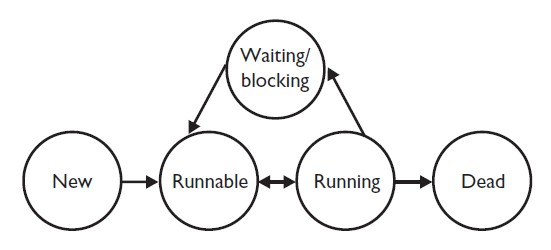
\includegraphics[scale=0.5]{Images/thread_states}
\end{center}

\subsubsection{Preventing Thread Execution}
For the exam, we are interested in the following within the 
`Waiting/Blocked/Sleeping' state:
\begin{itemize}
    \item Sleeping
    \item Waiting
    \item Blocked because it needs an object's lock
\end{itemize}
\subsubsection{Sleeping}
The \verb#sleep(long millis)# method is a static method of the \verb#Thread# 
class. You use it to `slow a thread down' by forcing it to go into a sleep mode 
for at least the duration specified before coming back to the `runnable' state.  
Note that the \verb#sleep()# method can throw an \verb#InterruptedException# 
which is a checked exception. Remember that \verb#sleep()# is static and 
affects the currently executing thread -- do not be fooled into thinking that 
one thread can put another to sleep

\subsubsection{Thread Priorities and yield()}
Threads always run with a priority, usually represented as a number between 1 
and 10 (although in some cases, the range is less than 10). In most jvms, the 
scheduler uses thread priorities to help determine which thread to run. If a 
thread enters the `runnable' state and has a higher priority than any of the 
threads in the pool and a higher priority then the currently executing thread, 
the lower riority running thread will usually be moved back to the `runnable' 
state and the higher priority thread will be chosen to run. In most cases, the 
running thread will be of equal or greater priority than the highest priority 
thread in the pool. Never rely on thread priorities to guarantee the correct 
behaviour of code

A thread gets a default priority that is the same as the thread of execution 
that created it. You can set a thread's priority by callig the 
\verb#setPriority()# method on a thread instance. Although the default priority 
is 5, the \verb#Thread# class has the following constants (\verb#static final# 
variables) that define the range of thread priorities:
\begin{itemize}
    \item \verb#Thread.MIN_PRIORITY     (1)#
    \item \verb#Thread.NORM_PRIORITY    (5)#
    \item \verb#Thread.MAX_PRIORITY     (10)#
\end{itemize}

The static \verb#Thread.yield()# method is supposed to make the currently 
running thread go back to `runnable' to allow other threads of the same 
priority to be chosen to run. However, the \verb#yield()# method is not 
guaranteed to do what it claims, and even if \verb#yield()# does cause a thread 
to move from `running' back to `runnable', there is no guarantee that the same 
thread will not be chosen to run again. Note that invoking \verb#yield()# will 
never cuase a thread to enter the `Waiting/Sleeping/Blocked' state. At most, 
\verb#yield()# will cause a thread to go from `running' to `runnable', but it 
might also have no effect at all

\subsubsection{The join() Method}
The non-static \verb#join()# method of the \verb#Thread# class lets one thread 
`join onto the end' of another thread. If you have a thread \verb#B# that 
cannot do its work until another thread \verb#A# has completed, then you want 
thread \verb#B# to `join' thread \verb#A#. This means that thread \verb#B# will 
not become `runnable' until \verb#A# has finished (and entered into the `dead' 
state). You can also call one of the overloaded versions of \verb#join()# that 
takes a timeout duration. Note that if the timeout expires, the thread becomes 
`runnable' again. Note that the \verb#join()# method can throw an 
\verb#InterruptedException# which is a checked exception

\subsubsection{Summary of ways a thread can leave the `running' state}
\begin{itemize}
    \item A call to \verb#sleep()# -- Guaranteed to cause the current thread to 
    stop executing for at least the specified duration (although it might be 
    interrupted before the end of the duration)
    \item A call to \verb#yield()# -- No guarantee to do much of anything, 
    although typically it will cause the currently running thread to move back 
    to `runnable' so that a thread of the same priority can have the 
    opportunity to start running. Note that threads with higher priority should 
    be managed by the jvm
    \item A call to \verb#join()# -- Guaranteed to cause the current thread to 
    stop executing until the thread it joins with (in other works, the thread 
    it calls \verb#join()# on) completes, however, if the thread it's trying to 
    join with is not alive, the current thread will not need to back out
\end{itemize}

There are also the following scenarios in which a thread might leave the 
`running' state:
\begin{itemize}
    \item The tread's \verb#run()# method completes
    \item A call to \verb#wait()# on an object (note that we do not call 
    \verb#wait()# on a \verb#Thread#)
    \item A thread cannot acquire the lock on an object whose method code it is 
    attempting to run
    \item The thread scheduler can decide to move the current thread from 
    `running' to `runnable' in order to give another thread a chance to run
\end{itemize}

\subsection{Synchronising Code}
To protect data from being read/modified by multiple threads concurrently, you 
must do two things:
\begin{itemize}
    \item Mark the instance variables \verb#private#
    \item Synchronise the code that modifies the variables
\end{itemize}
Remember that you protect the variables in the normal way -- using an access 
modifier. It is the method code that you must protect to ensure only one thread 
at a time can be executing that code. This is done using the 
\verb#synchronized# keyword

\subsubsection{Synchronisation and Locks}
Synchronisation works through locks. Every object in java has a build-in lock 
that only comes into play whent the object has synchronised method code. When a 
thread enters a synchronised non-static method, it automatically acquires the 
lock associated with the current instance of the class whose code the thread is 
executing (the \verb#this# instance).

Since there is only one lock per object, if one thread has the lock, no other 
thread can obtain it until the first thread releases it. This means no other 
thread can enter the synchronised code (which means it cannot enter any 
synchronised method of that object) until the lock has been released.  
Typically, releasing a lock means that the thread holding the lock exits the 
synchronised method.

Remember the following key points about locking and synchronisation:
\begin{itemize}
    \item Only methods (or blocks) can be synchronized -- not variables or 
    classes
    \item Each object has just one lock
    \item Not all methods in a class need to be synchronised. A class can have 
    both synchronised and non-synchronised methods
    \item If two threads are about to execute a synchronised method in a class, 
    and both threads are using the same instance of the class to invoke the 
    method, only one thread at a time will be able to execute the method
    \item If a class has both synchronised and non-synchronised methods, 
    multiple threads can still access the class's non-synchronised methods
    \item If a thread goes to sleep, it holds any locks it has -- it does not 
    release them
    \item A thread can acquire more than one lock. Also note that if a thread 
    acquires a lock and then attempts to call a synchronised method on the same 
    object, there is no problem
    \item You can synchronise a block of code rather than a method:
        \begin{verbatim}
            class SyncTest {
                public void doStuff() {
                    System.out.println("not synchronised");
                    synchronized(this) {
                        System.out.println("synchronised");
                    }
                }
            }
        \end{verbatim}
\end{itemize}

When you sychronise a method, the object used to invoke the method is the 
object whose lock must be acquired. When you synchronise a block of code, you 
specify which object's lock you want to use as the lock. This gives you the 
ability to have more than one lock for code synchronisation with a single 
object

\subsubsection{Synchronising Static Methods}
\verb#static# methods can be synchronised. Since there is only one copy of the 
\verb#static# data you are trying to protect, you only need one lock per class 
to synchronise static methods -- a lock for the whole class. There is such a 
lock -- every class loaded in java has a corresponding instance of 
\verb#java.lang.Class# representing that class. There is nothing special you 
need to do to synchronise a \verb#static# method:
\begin{verbatim}
    class MyClass {
        static int count;

        public static synchronized int getCount() {
            return count;
        }
    }
\end{verbatim}
This method could be re-written to use a synchronised code block:
\begin{verbatim}
    class MyClass {
        static int count;

        public static int getCount() {
            synchronized(MyClass.class) {       // MyClass.class is a class literal
                return count;
            }
        }
    }
\end{verbatim}

\subsubsection{What Happens if a Thread Cannot Get the Lock?}
If a thread tries to enter a \verb#synchronized# method but the lock is already 
taken, the thread is said to be blocked on the object's lock. Essentially, the 
thread goes into a kind of pool for that particular object and has to wait 
until the lock is released and the thread can again enter the 
`runnable/running' state.  When thinking about blocking, it is important to pay 
attention to which objects are being used for locking:
\begin{itemize}
    \item Threads calling non-\verb#static synchronixed# methods in the same 
    class will only block each other if they are invoked using the same 
    instance, since they each lock on the \verb#this# instance
    \item Threads calling \verb#static synchronized# methods in the same class 
    will always block each other, since they all lock on the same \verb#Class# 
    instance
    \item A \verb#static synchronized# method and a non-\verb#static synchronized# method will never block each other since they lock on 
    different objects
    \item For \verb#synchronized# blocks, you need to look at exactly what 
    object has been used for locking. Threads that synchronise on the same 
    object will block each other
\end{itemize}

Summary of thread related methods and lock behaviour:
\begin{center}
\begin{tabular}{lll}
    \textbf{Give Up Locks} & \textbf{Keep Locks} & \textbf{Class Defining the 
    Method} \\
    \hline
    \verb#wait()# & \verb#notify()#* & \verb#java.lang.Object# \\
    & \verb#join()# & \verb#java.lang.Thread# \\
    & \verb#sleep()# & \verb#java.lang.Thread# \\
    & \verb#yield()# & \verb#java.lang.Thread# \\
\end{tabular}
\end{center}
*Note that \verb#notify()# will probably exit the synchronised code shortly 
after this call and therefore give up its locks

\subsubsection{When Do You Need to Synchronise?}
Generally, any time more than one thread is accessing mutable data, you 
synchronise to protect that data, to ensure the threads are not changing it at 
the same time (or that one is not changing it at the same time the other is 
reading it).

Access to static fields should be done from static synchronised methods. Access 
to non-static fields should be done from non-static synchronised methods

\subsubsection{Thread-Safe Classes}
When a class has been carefully synchronised to protect its data, we say it is 
`thread-safe'. However, even when a class is `thread-safe', it is often 
dangerous to rely on these classes to provide the thread protection you need.  
The method \verb#Collections.synchronizedList()# returns a \verb#List# whose 
methods are all \verb#synchronized# and `thread-safe' according to the 
documentation. Note that in a `thread-safe' class (like the one returned by 
\verb#synchronizedList()#, each individual method is synchronised. So calls to 
\verb#size()# and \verb#remove()# for example are synchronised. However, 
nothing prevents another thread from doing something else to the list between 
the two calls, meaning problems can still occur. The simple solution is not to 
rely on `thead-safe' classes and synchronise the code yourself. Once you do 
that, the original synchronisation (in this case, the synchronisation inside 
the object returned by \verb#Collections.synchronizedList()#) may well become 
redundant

\subsubsection{Thread Deadlock}
Deadlock occurs when two threads are blocked, with each waiting for the other's 
lock. Neither can run until the other gives up its lock, so they will sit there 
forever

\subsection{Thread Interaction}
Using \verb#Object.wait()# and \verb#Object.notify()# lets one thread put 
itself into a `waiting room' until some other thread notifies it that there is 
a reason to come back out. Note that \verb#wait()#, \verb#notify()# and 
\verb#notifyAll()# must be called from within a synchronised context. A thread 
cannot invoke a \verb#wait()# or \verb#notify()# method on an object unless it 
owns the object's lock (otherwise an \verb#IllegalMonitorStateException# is 
thrown at runtime).

Remember that \verb#wait()# and \verb#notify()# are instance methods of 
\verb#Object#. In the same way that every object has a lock, every object can 
have a list of threads that are waiting for a notification from the object. A 
thread gets on this waiting list by invoking executing the \verb#wait()# method 
of the target object. From that moment, it does not execute any further until 
the \verb#notify()# (or \verb#notifyAll()#) method of the target object is 
called (and the thread is chosen by the thread scheduler to run). If multiple 
threads are waiting on the same object, \verb#notify()# will cause only one to 
be chosen (in no guaranteed order) to proceed with its execution. If there are 
no threads waiting, then no particular action is taken.

When a thread waits, it temporarily releases the lock for other threads to use, 
but it will need it again to continue execution. It is common to find code like 
this:
\begin{verbatim}
    synchronized(anotherObject) {   // this has the lock on anotherObject
        try {
            anotherObject.wait();
            // the thread releases the lock and waits. To continue, the thread 
            // needs the lock, so it may be blocked until it gets it
        }
        catch(InterruptedException e) {}
    }
\end{verbatim}
The preceeding code waits until \verb#notify()# (or \verb#notifyAll()#) is 
called on \verb#anotherObject#:
\begin{verbatim}
    synchronized(this) {
        notify();
    }
\end{verbatim}
This code notifies a single thread currently waiting on the \verb#this# object.
The lock can be acquired much earlier in the code, such as in the calling 
method. Note that if the thread calling \verb#wait()# does not own the lock, it 
will throw an \verb#IllegalMonitorStateException#. This is not a checked 
exception, so you do not need to catch it explicitly. You should always be 
clear whether a thread has the lock of an object in any given block of code.

Note that \verb#wait()# was called from within a try-catch block. A waiting 
thread can be interrupted in the same way as a sleeping thread, so you need to 
handle the exception.

There is an overloaded version of \verb#wait()# that accepts a number of 
milliseconds as a maximum time to wait. If the thread is not interrupted, it 
will continue normally whenever it is notified or the specified timeout has 
elapsed. This normal continuation consists of getting out of the waiting state, 
but to continue execution, it will have to get the lock for the object.

When the \verb#wait()# method is invoked on an object, the thread executing 
that code gives up its lock on the object immediately. However, when 
\verb#notify()# is called, that does not mean the thread gives up its lock at 
that moment. If the thread is still completing synchronised code, the lock is 
not released until the thread moves out of the synchronised code

\subsubsection{Using notifyAll() When Many Threads May Be Waiting}
In most scenarios, it is preferable to notify all of the threads that are 
waiting on a particular object. If so, you can use \verb#notifyAll()# on the 
object to let all the threads rush out of the `waiting' state and back to 
`runnable'. This is especially important if you have several threads waiting on 
one object, but for different reasons, and ou want to be sure that the right 
thread (along with all the others) gets notified.

Using \verb#notifyAll()# means that all the notified threads will start 
competing to get the lock. As the lock is used and released by each thread, all 
of them will enter into action without a need for further notification.  
Remember that using \verb#notify()# will only affect one of the possibly many 
waiting threads. Which one depends on jvm implementation, and so program 
correctness should never rely upon one thread being notified in preference to 
another

\subsubsection{Using wait() in a Loop}
If a call to \verb#notify()# happens before the corresponding call to 
\verb#wait()#, the thread which calls \verb#wait()# will continue to wait for a 
notification but might never receive it, since it has already occurred. This 
situation is probably not what was intended. Almost always, when you want to 
wait for something, you also need to be able to check if it has already 
happened. Generally, the best way to solve this is to use a loop that checks on 
a conditional expression, and only waits if the thing you are waiting for has 
not yet happened.

There is also a possible situation called `spontaneous wakeup' that may exist 
in some situations -- a thread may wake up even though no code has called 
\verb#notify()# or \verb#notifyAll()#. At least, no code you know about has 
called these methods. Sometimes the jvm may call \verb#notify()# for reasons of 
its own, or code in some other class calls it for reasons you just do not know.
What this means is, when your thread wakes up from a \verb#wait()#, you do not 
know for sure why it was awoken. By puttig the \verb#wait()# invocation in a 
\verb#while# loop and re-checking the condition that represents what we were 
waiting for, we ensure that whatever the reason we woke up, we will re-enter 
the \verb#wait()# if the thing we were waiting for has not happened yet. 

The moral here is that when you use \verb#wait()# and \verb#notify()# or 
\verb#notifyAll()#, you shoud almost always also have a \verb#while# loop 
around the \verb#wait()# that checks a condition and forces continued waiting 
until the condition is met. You should also make use of the required 
synchronisation for the \verb#wait()# and \verb#notify()# calls, to protect 
whatever data you are sharing between threads. If you see code which fails to 
do this, there is usually something wrong with the code -- even if you have a 
hard time spotting what it is

\subsubsection{Summary of Key Thread Related Methods}
\begin{center}
\begin{tabular}{lll}
    \textbf{Class Object} & \textbf{Class Thread} & \textbf{Interface Runnable} 
    \\
    \hline
    \verb#wait()# & \verb#start()# & \verb#run()# \\
    \verb#notify()# & \verb#yield()# & \\
    \verb#notifyAll()# & \verb#sleep()# & \\
    & \verb#join()# & \\
\end{tabular}
\end{center}
